\documentclass[xcolor=table]{beamer}

\usepackage{lscape, amsmath, amsfonts, amssymb, setspace, theorem, wrapfig, graphicx, float, multirow, subfig, color, rotating, multicol, datetime, natbib, venndiagram, pstricks, xkeyval, tikz, etoolbox, url, hyperref, nth}

\usepackage[T1]{fontenc}
\usepackage[latin1]{inputenc}
\usepackage[english]{babel}
\usetikzlibrary{arrows,calc,matrix}

\title{GV217 - Conflict Analysis}
\subtitle{University of Essex - Department of Government}
\date{Week 23 -- 6 March, 2020}				% or you can specify a date, just write it down instead of "\today"
\author{Lorenzo Crippa} 

\usetheme[progressbar=frametitle]{metropolis}
\usecolortheme{seahorse}						% try others: wolverine; crane...

\begin{document}
\frame{
\titlepage
}

\begin{frame}{2020 Department of Government Student Conference}
\centering

\includegraphics[scale=0.35]{pictures/week_23_conference.pdf} 
\end{frame}

\section{Ethnic conflicts}

\begin{frame}{What is ethnicity?}
Ethnicity is a group identity based on shared customs, language, history, often religion\ldots \pause

Debate: \pause
\begin{enumerate}
\item Is ethnicity a permanent feature of groups? \pause
\item Is ethnicity socially constructed? \pause
\end{enumerate}

The answer we give to this debate has relevant implications for the solution to ethnic conflicts
\end{frame}

\begin{frame}{What is ethnic conflict?}
\begin{itemize}
\item ``Ethnic conflict encompasses all forms of small- and large-scale acts of violence between and among different ethnic groups.'' \pause
\item ``An ethnic group is a group of people that belong to a certain ascriptive category, such as race, ethnicity, language, tribe, religion, and so forth.''
\end{itemize}
(Brancati 2006: 654)
\end{frame}

\begin{frame}{What causes ethnic conflicts?}
\textcolor{red}{Assumption: Violence is costly for all actors} \\ \pause
Knowing the causes of ethnic conflict is the first step to devise solutions. We can identify some causes of ethnic conflicts (Lake and Rothchild 1996): \pause
\begin{enumerate}
\item Bargaining issues \pause
	\begin{itemize}
	\item Asymmetry of information (incentives to misrepresent) \pause
	\item Commitment problems \pause
	\end{itemize}
\item Security dilemma \pause
	\begin{itemize}
	\item One's increase in security makes the other less secure \pause
	\end{itemize}
\item Breakdown of government institutions \pause
	\begin{itemize}
	\item Regime fall \pause
	\item New, weak democracy \pause
	\item Opportunities for ethnic divisions to emerge
	\end{itemize}
\end{enumerate}
\end{frame}

\begin{frame}[fragile]
\frametitle{Security dilemma}
Drawn from game theoretic Prisoner's Dilemma Game (PDG): \pause
\begin{itemize}
\item Two rational players can Arm or Disarm \pause
\item Optimal equilibrium impossible to reach \pause
\item Suboptimal Nash equilibrium \pause
\end{itemize}

\begin{table}[h]
\centering
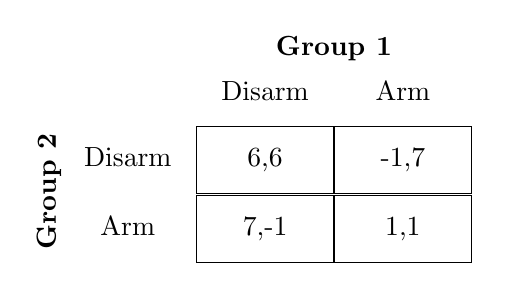
\begin{tikzpicture}[element/.style={minimum width=1.75cm,minimum height=0.85cm}]
\matrix (m) [matrix of nodes,nodes={element},column sep=-\pgflinewidth, row sep=-\pgflinewidth,]{
         & Disarm  & Arm  \\
Disarm & |[draw]|6,6 & |[draw]|-1,7 \\
Arm & |[draw]|7,-1 & |[draw]|1,1 \\    };


\node[above=0.25cm] at ($(m-1-2)!0.5!(m-1-3)$){\textbf{Group 1}};
\node[rotate=90] at ($(m-2-1)!0.5!(m-3-1)+(-1,0)$){\textbf{Group 2}};
\end{tikzpicture}
\end{table}
\end{frame}

\begin{frame}{Causal interconnections}
\centering
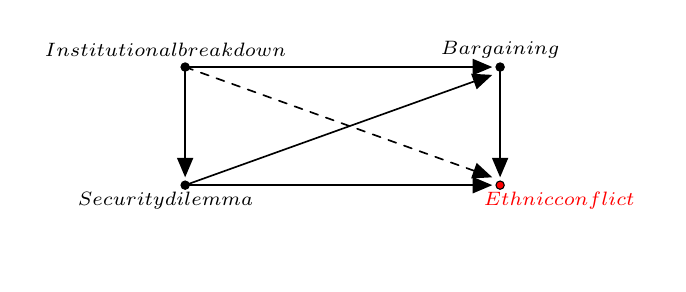
\begin{tikzpicture}[line cap=round,line join=round,>=triangle 45,x=1cm,y=1cm]
\clip(-3,-1) rectangle (5,2);
\draw [dashed,->,line width=0.6pt] (-1,1.5) -- (2.9,0.1);
\draw [->,line width=0.6pt] (-1,1.5) -- (-1,0.1);
\draw [->,line width=0.6pt] (-1,1.5) -- (2.9,1.5);
\draw [->,line width=0.6pt] (-1,0) -- (2.9,0);
\draw [->,line width=0.6pt] (3,1.5) -- (3,0.1);
\draw [->,line width=0.6pt] (-1,0) -- (2.9, 1.4);
\begin{scriptsize}
\draw [fill=black] (-1,1.5) circle (1.5pt);
\draw[color=black] (-1.25,1.72) node {$Institutional{}breakdown$};
\draw [fill=black] (-1,0) circle (1.5pt);
\draw[color=black] (-1.25,-0.2) node {$Security{}dilemma$};
\draw [fill=red] (3,0) circle (1.5pt);
\draw[color=red] (3.75,-0.2) node {$Ethnic{}conflict$};
\draw [fill=black] (3,1.5) circle (1.5pt);
\draw[color=black] (3,1.72) node {$Bargaining$};
\end{scriptsize}
\end{tikzpicture} \\ \pause
Example: Iraq after 2003 \pause
\begin{itemize}
\item Iraq was ruled by Saddam Hussein's Sunni (minority) dictatorship until 2003, a repressive but stable regime \pause
\item After the invasion of the coalition and the regime fall, a weak democratic regime was established \pause
\item This created a security dilemma among ethnic groups \pause
\item The two causes combined contributed to the ethnic conflict
\end{itemize}
\end{frame}

\begin{frame}{Security dilemma and marginalization, Baghdad 2003}
\begin{figure}
\centering
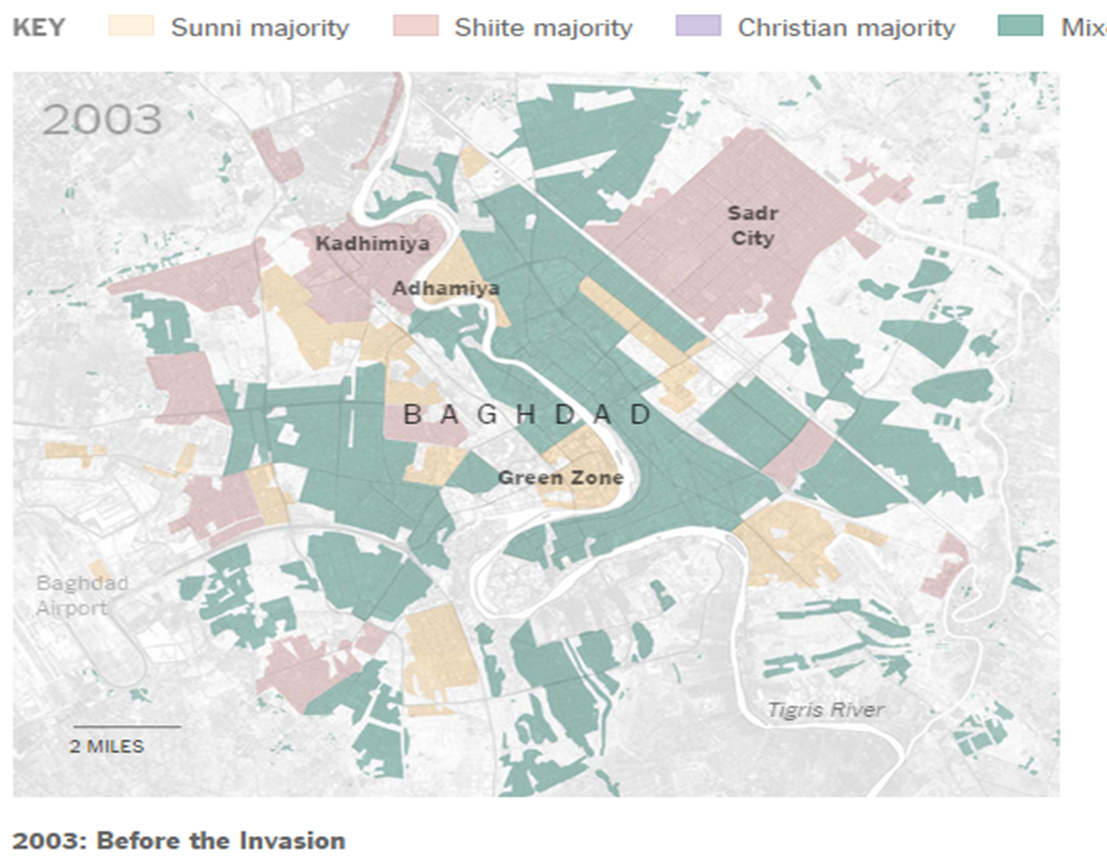
\includegraphics[scale=.45]{pictures/week23_baghdad1.png}
\caption{Source: NY Times}
\end{figure}
\end{frame}

\begin{frame}{Security dilemma and marginalization, Baghdad 2009}
\begin{figure}
\centering
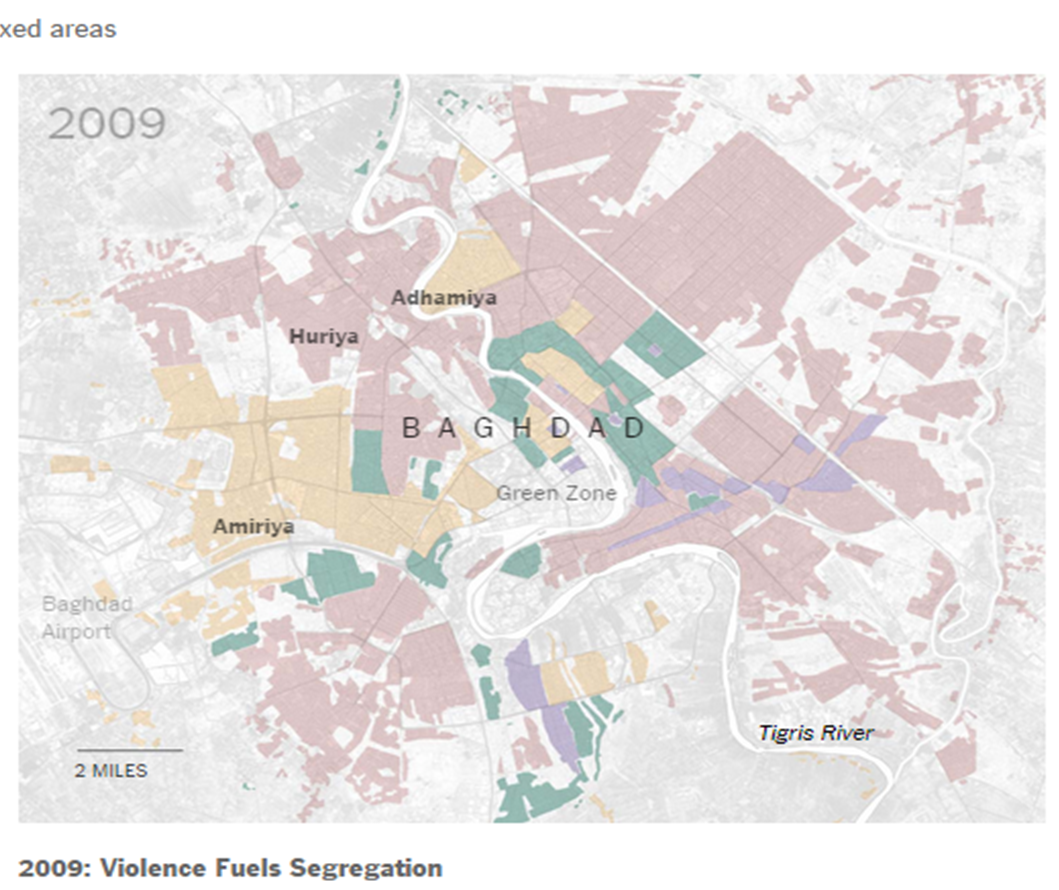
\includegraphics[scale=.45]{pictures/week23_baghdad2.png}
\caption{Source: NY Times}
\end{figure}
\end{frame}

\begin{frame}{What hypotheses about ethnic conflicts?}
We can derive a few hypotheses from these points: \pause
\begin{enumerate}
\item[H1] Ethnic marginalisation and segregation increases the probability of ethnic conflicts \pause
	\begin{itemize}
	\item[H1.a] Separated ethnic groups that increase security measures increase the probability of ethnic conflicts \pause
	\end{itemize}
\item[H2] Regime fall in contexts of ethnic divisions increases the probability of ethnic conflicts \pause
	\begin{enumerate}
	\item[H2.a] Weak democracies in contexts of ethnic divisions increases the probability of ethnic conflicts \pause
	\item[H2.b] New democracies in contexts of ethnic divisions increases the probability of ethnic conflicts
	\end{enumerate}
\end{enumerate}
\end{frame}

\begin{frame}{Case study: Rwanda}
\begin{itemize}
\item Divide in groups of 2-3 people
\item Discuss the following questions based on the handout
\end{itemize} \pause

\begin{enumerate}
\item Is ethnicity in Rwanda a primordial feature or was it socially constructed? \pause
\item How would you explain the onset of the conflict and its escalation to genocide? \pause
\item What role did ethnicity play? \pause
\item Does the explanations we have proposed apply?
\end{enumerate}
\end{frame}

\begin{frame}{Solutions of ethnic conflict}
\begin{itemize}
\item Reassure minority groups of their physical and cultural safety (Lake and Rothchild 1996) \pause
\item International partition of disputed areas \pause
	\begin{itemize}
	\item[--] Risks turning a civil conflict into an interstate one \pause
	\item[--] Risks new ethnic civil conflicts (\textit{e.g.} former Yugoslavia)
	\end{itemize} \pause
\item Decentralization of national government (Brancati 2006) \pause
\item Power-sharing; granting group rights (Gleditsch et al. 2017)
\end{itemize}
\end{frame}

%\begin{frame}{Trends}
%\centering
%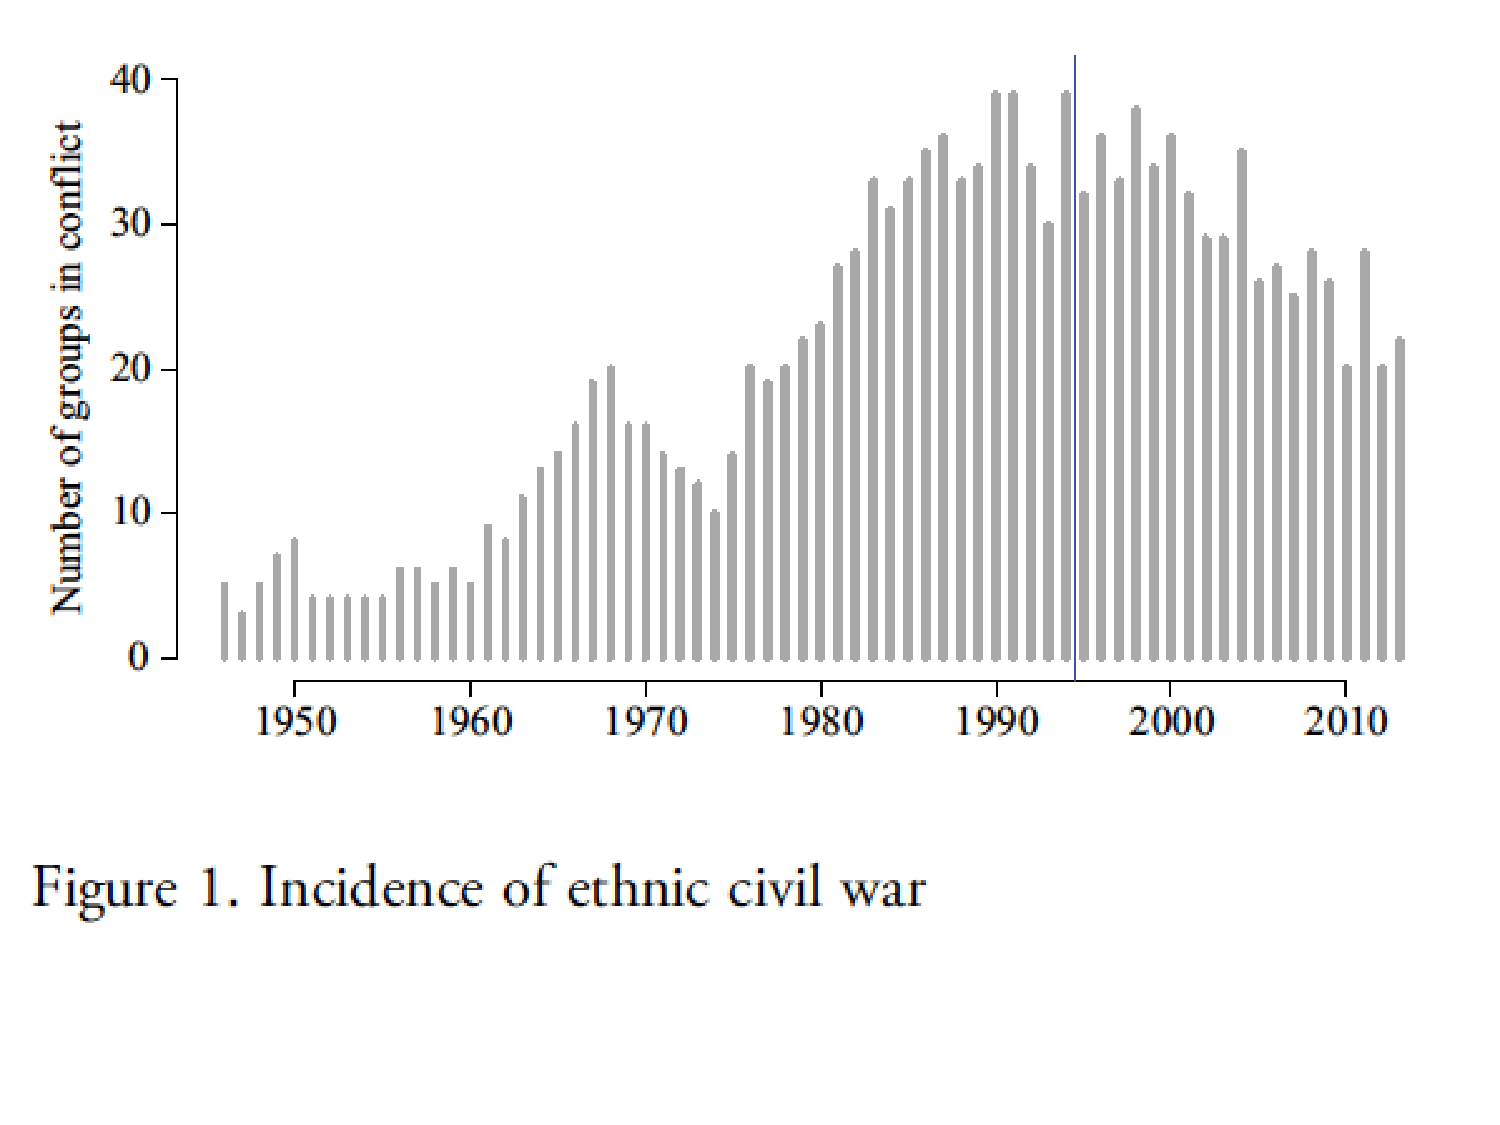
\includegraphics[scale=.4]{pictures/week_23_1.pdf} 
%\end{frame}

%\begin{frame}{Trends}
%\centering
%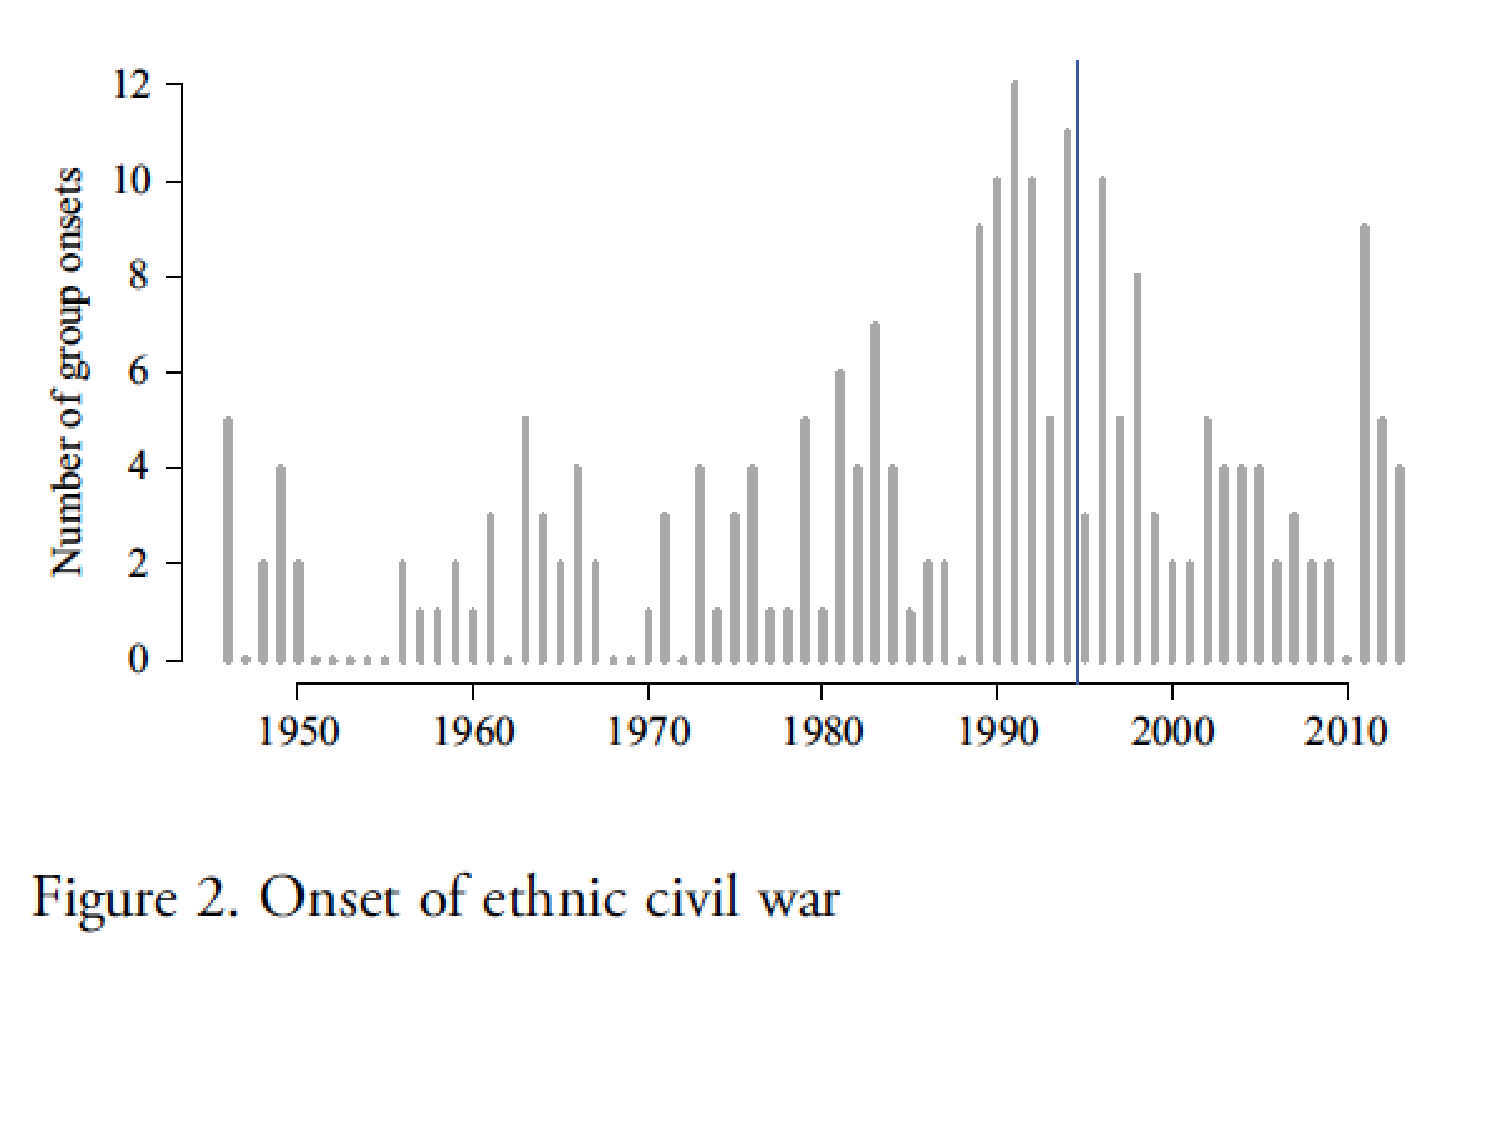
\includegraphics[scale=.4]{pictures/week_23_2.pdf} 
%\end{frame}

%\begin{frame}{Trends}
%Decline since mid 1990s (end of Cold War) 

%Why? Granting of group rights, regional autonomy, and inclusion in power-sharing, as well as democratization and peacekeeping

%$\rightarrow$ role of grievances for conflict and the potential for accommodation to help settle conflicts

%Thoughts? What make ethnicity so important in conflicts?
%\end{frame}

\frame{
\frametitle{Conclusion}
\begin{center}
All clear? More questions? \\
See you next week!
\end{center}
}

\end{document}